\documentclass[aps,prb,superscriptaddress,nofootinbib]{revtex4}
\usepackage{amsfonts}
\usepackage{amsmath}
\usepackage{amssymb}
\usepackage{graphicx}
\usepackage{graphbox}
\usepackage{caption}
\usepackage{bm}
\usepackage{bbm}
\usepackage{cancel}
\usepackage{color}
\usepackage{mathrsfs}
\usepackage[colorlinks,bookmarks=true,citecolor=blue,linkcolor=red,urlcolor=blue]{hyperref}
\usepackage{simpler-wick}
\usepackage{appendix}
\usepackage{float}
\usepackage{sleek-listings}
\usepackage{array}
\usepackage{booktabs}
\setlength{\parindent}{10 pt}
\setlength{\parskip}{2 pt}
\setcounter{MaxMatrixCols}{30}
\bibliographystyle{apsrev}

\newcommand{\normord}[1]{{:\mathrel{#1}:}}
\def\tbs{\textbackslash}
\def \tr{\operatorname{tr}}
\def \Tr{\operatorname{Tr}}


\begin{document}
\title{Phi-4 Theory}
\author{Jie Ren}

\FrameTBStyle{mathematica}

\maketitle



\tableofcontents

\section{Quantization}
We study the interacting scalar field theory with the $\phi^4$ interaction.
\begin{equation*}
	\mathcal L = \mathcal L_\text{K-G} + \mathcal L_{\mathrm{int}}
	= \frac{1}{2}\partial^\mu \phi \partial_\mu \phi -\frac{m^2}{2}\phi^2 -\frac{g}{4!}\phi^4.
\end{equation*}
Note that the theory has the $Z_2$ symmetry: $\phi \rightarrow -\phi$, 


\subsection{Canonical quantization}
The equation of motion\footnote{The equation of motion for a classical field is: $\partial_\mu \left[\frac{\partial \mathcal L}{\partial(\partial_\mu \phi)}\right] - \frac{\partial \mathcal L}{\partial \phi} = 0$.} the Klein-Gordon Lagrangian is $(\partial_t^2-\nabla^2+m^2)\phi(\bm x,t) = 0$.
The (classical) solutions are the plane waves: $\phi_{\bm k}(\bm x, t) \propto e^{-i\omega_{\bm{k}}t+i\bm{k}\cdot\bm{x}} + e^{i\omega_{\bm{k}}t-i\bm{k}\cdot\bm{x}}$, where $\omega_{\bm{k}}=\bm{k}^2+m^2$.
The general solution can be
\begin{equation*}
	\phi(\bm x,t) = \int \frac{d^{3} k}{(2\pi)^{3}} \left(
		a_{k}e^{-i\omega_{\bm{k}}t+i\bm{k}\cdot\bm{x}} + 
		a^*_{k}e^{i\omega_{\bm{k}}t-i\bm{k}\cdot\bm{x}} 
	\right),
\end{equation*}
where $a_k$'s are arbitrary c-numbers.
The \textit{quantization} is the procedure to discretize the coefficient $a_k$'s.
The \textit{canonical} way to do it is to promote the coefficient $a_{k}/a_{k}^*$ to the particle annihilation/creation operator $a_{k}/a_{k}^\dagger$, with the commutation relation
\begin{equation}
	[a_{k}, a_{p}^\dagger] = (2\pi)^{3} \delta^{3}(\bm{k}-\bm{p}).
\end{equation}
The single-particle state with momentum $\bm k$ is created by $a_{k}^{\dagger}$ operators acting on the vacuum.

\

\noindent\textbf{Claim:}
A natural choice of the normalization convention is to set
\begin{equation}
	|\bm{k}\rangle \equiv \sqrt{2\omega_{\bm k}} a_{k}^{\dagger}|0\rangle,
	\label{eq:rel-single-particle}
\end{equation}
in order to ensure the Lorentz invariant.

\noindent\textit{Proof:}
We first note that the following expression is Lorentz invariant and serve as a proper candidate for the identity operator:
\begin{equation*}
	\hat P = \int \frac{d^{3} p}{(2\pi)^{3}} \frac{|\bm{p}\rangle\langle\bm{p}|}{2\omega_{\bm p}}
	=2\pi \int \frac{d^{3} p d\omega}{(2\pi)^{4}} \delta(\omega^2-{\bm{p}}^2-m^2) |\bm p\rangle\langle \bm p|.
\end{equation*}
If we fix the convention by $\hat P = \hat{\mathbb I}$, we will need the following equality to hold:
\begin{equation*}
	|\bm{k}\rangle
	=\int \frac{d^{3} p}{(2\pi)^{3}} \frac{\langle\bm{p}|\bm{k}\rangle}{2\omega_{\bm p}}|\bm{p}\rangle 
	\quad \Longleftrightarrow \quad
	\langle\bm{p}|\bm{k}\rangle 
	= 2\omega_{\bm p}(2\pi)^3 \delta^3(\bm{p}-\bm{k})
	=|\bm{k}\rangle.
\end{equation*}
This definition of inner product comes from Eq.~(\ref{eq:rel-single-particle}):
\begin{equation*}
	\langle\bm{p}|\bm{k}\rangle 
	= 2\sqrt{\omega_{\bm p} \omega_{\bm k}}\left\langle 0\left|a_{p} a_{k}^{\dagger}\right| 0\right\rangle
	= 2 \omega_{\bm p}(2\pi)^{3} \delta^{3}(\bm{p}-\bm{k}).
\end{equation*}

\noindent\textit{Remark:}
The single-particle defined above can be used to fix the normalization $\langle \bm k|\phi(\bm x,0)|0\rangle = e^{-i \bm k\cdot \bm x}$, leading to the field expansion
\begin{equation}
	\phi(x)
	=\int \frac{d^{3} k}{(2\pi)^{3}} \frac{1}{\sqrt{2\omega_{\bm k}}}\left(a_k 
		e^{-i k \cdot x}+a_k^{\dagger} e^{i k \cdot x}\right).
\end{equation}

\

\noindent\textbf{Claim:}
We can obtain the Hamiltonian for the Klein-Gordon field using the Legendre transformation:
\begin{equation}
	H = \int d^4 x\ \left[\pi(x) \dot{\phi}(x) - \mathcal L(x) \right] 
	= \int d^4 x\ \frac{1}{2} \left[\pi^2 + (\nabla \phi)^2 + m^2 \phi^2 \right],
\end{equation}
where the canonical momentum is defined as
\begin{equation}
	\pi(x) = \frac{\partial \mathcal L}{\partial \dot{\phi}} = \dot{\phi}(x) 
	= -i\int \frac{d^{3} k}{(2\pi)^{3}} \sqrt{\frac{\omega_{k}}{2}}\left(a_k 
		e^{-i k \cdot x} - a_k^{\dagger} e^{i k \cdot x}\right).
\end{equation}

\noindent\textit{Proof:}
The $\pi^2$ term expands as
\begin{equation}
	\pi^2(x) = \int \frac{d^{3} k_1}{(2\pi)^{3}} \frac{d^{3} k_2}{(2\pi)^{3}}
		\frac{\sqrt{\omega_{k_1} \omega_{k_2}}}{2} \left(a^\dagger_{k_1}a_{k_2}e^{i(k_1-k_2)x} - a^\dagger_{k_1} a^\dagger_{k_2} e^{i(k_1+k_2)x} + h.c.\right).
\end{equation}
We note that after integrate over $x$, the phase factor $e^{i(k_1-k_2)x}$ produce a delta function for $k_1$ and $k_2$.
The $a^\dagger_{k_1} a^\dagger_{k_2}$ terms will finally be cancelled by other terms.
We temporally ignore such term.
The contribution from the first term is then
\begin{equation}
	\int d^4 x\ \pi^2(x) = \int \frac{d^3 k}{(2\pi)^3} \frac{\omega_k}{2} a_k^\dagger a_k + h.c.
\end{equation}
The second term is
\begin{equation}
	(\nabla \phi)^2 = \int \frac{d^{3} k_1}{(2\pi)^{3}} \frac{d^{3} k_2}{(2\pi)^{3}}
		\frac{\bm k_1 \bm k_2}{2\sqrt{\omega_{k_1}\omega_{k_2}}} \left(a^\dagger_{k_1}a_{k_2}e^{i(k_1-k_2)x} - a^\dagger_{k_1} a^\dagger_{k_2} e^{i(k_1+k_2)x} + h.c.\right).
\end{equation}
The third term is
\begin{equation}
	m^2 \phi^2 = \int \frac{d^{3} k_1}{(2\pi)^{3}} \frac{d^{3} k_2}{(2\pi)^{3}}
		\frac{m^2}{2\sqrt{\omega_{k_1}\omega_{k_2}}} \left(a^\dagger_{k_1}a_{k_2}e^{i(k_1-k_2)x} + a^\dagger_{k_1} a^\dagger_{k_2} e^{i(k_1+k_2)x} + h.c.\right).
\end{equation}
All three contributions sum up as
\begin{equation}
	H = \int \frac{d^3 k}{(2\pi)^3} \frac{1}{2}\left(\frac{\omega_k}{2} + \frac{\bm k^2+m^2}{2 \omega_k}\right) \left(a_k^\dagger a_k + h.c. \right) 
	= \int \frac{d^3 k}{(2\pi)^3} \omega_k \left(a_k^\dagger a_k +\frac{1}{2} \right).
\end{equation}
We can now check that the $a^\dagger a^\dagger$ terms indeed have no contributions, as the total contribution for each momentum $k$ is $-\frac{\omega_k}{2} + \frac{\bm k^2}{2\omega_k} + \frac{m^2}{2\omega_k} = 0$.
The Hamiltonian in the operator form also makes it manifest that $H |\bm k\rangle = \omega_k |\bm k\rangle$.

\

\noindent\textbf{Claim:}
The propagator of the free field is
\begin{equation}
	i\Delta(k) = \frac{i}{k^2-m^2+i\epsilon}
\end{equation}

\noindent\textit{Proof:}
Consider the two-point correlation:
\begin{equation}
	i\Delta(x_1-x_2) \equiv \langle 0|T \phi(x_1) \phi(x_2) |0\rangle 
	= \theta(t_1-t_2) \langle 0|\phi(x_1) \phi(x_2) |0\rangle 
	+ \theta(t_2-t_1) \langle 0|\phi(x_2) \phi(x_1) |0\rangle.
\end{equation}
Note that
\begin{equation}
	\langle 0|\phi(x_1) \phi(x_2) |0\rangle
	= \int\frac{d^{3} k}{(2\pi)^{3}}\frac{1}{2\omega_k} e^{i\bm k\cdot (\bm x_1-\bm x_2)-i\omega_{\bm k}\tau},
\end{equation}
where $\tau =t_1-t_2$.
The propagator can be written as\footnote{We need the identity
\begin{equation*}
	\frac{1}{2\omega_k} \left[e^{-i\omega_{\bm k}\tau}\theta(\tau)+e^{i\omega_{\bm k}\tau}\theta(-\tau)\right] 
	= \int \frac{d\omega}{2\pi i} \frac{-e^{i\omega\tau}}{\omega^2-\omega_k^2+i\epsilon},
\end{equation*}
where an infinitesimal number $\epsilon$ is included to move the singularities away from the real axis.}
\begin{eqnarray}
	i\Delta(x_1-x_2) 
	&=& \int\frac{d^{3} k}{(2\pi)^{3}}\frac{e^{i\bm k\cdot (\bm x_1-\bm x_2)}}{2\omega_k} \left[e^{-i\omega_{\bm k}\tau}\theta(\tau)+e^{i\omega_{\bm k}\tau}\theta(-\tau)\right] 
	= \int\frac{d^{3} k}{(2\pi)^{3}} \int \frac{d\omega}{2\pi i}\frac{-e^{i\bm k\cdot (\bm x_1-\bm x_2)+i\omega\tau}}{\omega^2-\omega_k^2+i\epsilon} \nonumber\\
	&=& \int\frac{d^{4} k}{(2\pi)^{4}} e^{-i k\cdot (x_1-x_2)}\frac{i}{k^2-m^2+i\epsilon},
\end{eqnarray}
Any final result shall take the ($\epsilon \rightarrow 0^+$) limit.
Sometimes the infinitesimal $\epsilon$ will be absorbed into the mass, i.e., $m^2 \rightarrow m^2-i\epsilon$.


\subsection{Path integral formalism}
Consider the action for free field with source
\begin{equation}
	S[\phi,J]
	= \int d^dx\left[\mathcal{L}(\phi) + J(x)\cdot\phi(x) \right].
\end{equation}
In the path integral formalism, we consider the partition function with source: $Z[J] = \int D[\phi]\ e^{iS[\phi,J]}$.
The central quantity a field theory produces is the correlation function of field values at different spacetime points $iG(x_1,\cdots,x_n) \equiv \langle \phi(x_1)\cdots \phi(x_n)\rangle$, where $\langle \cdots \rangle$ denotes the (time-ordered) average defined by the functional integral:
\begin{equation}
	\langle \cdots \rangle \equiv \frac{1}{Z[0]}\int D[\phi]\ e^{-iS[\phi]} (\cdots).
\end{equation}
We see that the partition function produces all possible correlation functions:
\begin{equation}
	iG(x_1,\cdots,x_n) = \left. \prod_{i=1}^n \left[\frac{\delta}{i\delta J(x_i)}\right] Z[J] \right|_{J=0}.
\end{equation}
The partition function $Z[J]$ is thus a generating functional.
For interaction theory, the perturbation approach is that we first evaluate the generating functional for free field $Z_0[J]$, then the generating functional for interacting field can be formally expressed as:
\begin{equation}
	Z[J] = \exp\left(i\int d^dx \mathcal{L}_{\mathrm{int}}\left[\frac{\delta}{i\delta J(x)}\right]\right)Z_0[J],
\end{equation}
which can then be Taylor expanded order by order.
Since the unconnected diagram can be absorbed into $Z[0]$, we only need to calculate the connected diagrams.
The procedure of perturbative expansion with only connected diagrams can be formally represented by introducing the quantity $Z[J] = Z[0]\exp\left(i W[J]\right)$.
The perturbative expansion of $W[J]$ contains only the connected diagrams.
Note that for the free theory,
\begin{equation*}
	\frac{Z_0[J]}{Z_0[0]} = \exp\left[-\frac{i}{2}\int d^d x_1 d^d x_2 J(x_1) \Delta(x_1-x_2)J(x_2)\right],
\end{equation*}
which means $W_0 = -\frac{1}{2}\int d^d x_1 d^d x_2 J(x_1) \Delta(x_1-x_2)J(x_2)$.
Consider the four-point connected correlation $iG^c_4$.
Following the same procedure,
\begin{equation*}
	iG^c_4 
	= i\left.\frac{\delta^4 W[J]}{i\delta J(x_1)i\delta J(x_2)i\delta J(x_3)i\delta J(x_4)}\right|_{J=0} 
	= \frac{1}{Z[0]}\left.\frac{\delta^4 Z[J]}{i\delta J_1 i\delta J_2 i\delta J_3 i\delta J_4}\right|_{J=0} 
	-i\Delta_{1,2} i\Delta_{3,4} -i\Delta_{1,3} i\Delta_{2,4} -i\Delta_{1,4} i\Delta_{2,3}.
\end{equation*}
The connected correlation function automatically omits those disconnected components.

Now we evaluate the propagator in the path-integral formalism.
In momentum space, the free action (with source) is\footnote{The space-time Fourier transformation is: 
\begin{equation*}
	\tilde{f}(k) = \int d^{d}x\ e^{ik\cdot x} f(x),\quad
	f(x) = \int \frac{d^{d}k}{(2\pi)^{d}}\ e^{-ik\cdot x}\tilde{f}(k),
\end{equation*}
where the inner product of two $d$-vectors is defined as $a \cdot b = a^0 b^b - \bm a \cdot \bm b$.}
\begin{equation*}
	\frac{1}{V}\sum_k \left[\frac{1}{2}\tilde\phi^*(k)( k^2-m^2)\tilde\phi(k)+\tilde J^*(k)\cdot\tilde\phi(k)+\tilde\phi^*(k)\cdot\tilde J(k)\right].
\end{equation*}
For real field, $\tilde\phi^*(k) = \tilde\phi(-k)$.
For our convenience, we have expressed the momentum integral as summation.
Actually, consider the $d$-dimensional box of size $L^d$, the momentum along each axis is multiple of $2\pi/L$, so when $L\rightarrow \infty$, the summation approaches in integral, $\frac{1}{V}\sum_k \rightarrow \int \frac{d^d k}{(2\pi)^d}$.
Let us omit the $1/V$ factor, the summation can be formally expressed as $\frac{1}{4}\mathbf{v}^T \cdot \mathbf M\cdot \mathbf{v} + \frac{1}{2}\mathbf{j}^T \cdot \mathbf{v}$, where
\begin{equation*}
	\mathbf v = \bigoplus_{|\mathbf k|} \left[
	\begin{array}{c}
		\tilde{\phi}(k) \\ 
		\tilde{\phi}^*(k) 
	\end{array}\right], \quad
	\mathbf M = \bigoplus_{|\mathbf k|} \left[
	\begin{array}{cc} 
		0 & k^2-m^2 \\ 
		k^2-m^2 & 0 
	\end{array}\right], \quad
	\mathbf j = \bigoplus_{|\mathbf k|} \left[
	\begin{array}{c}
		\tilde{J}^*(k) \\ 
		\tilde{J}(k) 
	\end{array}\right].
\end{equation*}
Note that in the above expression, we have made an infinitesimal shift of mass ($m^2 \rightarrow m^2 - i\epsilon$) to ensure the convergence of the Gaussian integral.
The integrated variables $v_i$ is not real.
To use the real Gaussian integral formula, we make use of a unitary transformation: 
\begin{equation*}
	\mathbf U = \frac{1}{\sqrt 2} \left[\begin{array}{cc}
		1 & 1 \\
		-i & i
	\end{array}\right], \quad
	\mathbf U \cdot \left[
	\begin{array}{c}
		\tilde{\phi}(k) \\ 
		\tilde{\phi}^*(k) 
	\end{array}\right] 
	= \frac{1}{\sqrt 2}\left[
	\begin{array}{c}
		\tilde\phi(k)+\tilde\phi^*(k) \\ 
		-i\tilde\phi(k)+i\tilde\phi^*(k)
	\end{array}\right]
	\equiv \left[
	\begin{array}{c}
		\tilde\phi_1(k) \\ 
		\tilde\phi_2(k) 
	\end{array}\right]
\end{equation*}
The path integral then becomes a real field integral.
Recall the real Gaussian integral formula:
\begin{equation}
	\int d\mathbf x \exp\left(-\frac{1}{2}\mathbf{x}^T \cdot \mathbf A \cdot \mathbf{x} + \mathbf{B}^T \cdot \mathbf{x}\right) 
	= \sqrt{\frac{(2\pi)^N}{\det{\mathbf A}}}\exp\left(\frac{1}{2}\mathbf{B}^T \cdot \mathbf{A}^{-1} \cdot \mathbf{B}\right),
	\label{eq:real-gaussian-integral}
\end{equation}
For the field integral, we absorbed the $(2\pi)^{N/2}$ term into the measure, and express the path integral for the Gaussian field as:
\begin{equation}
	W_0[J] 
	= -\frac{i}{4}\int \frac{d^d k}{(2\pi)^d} \mathbf j^T_k \cdot \mathbf M^{-1}_k \cdot \mathbf j_k
	= -\frac{1}{2} \int \frac{d^d k}{(2\pi)^d}  \tilde{J}^*(k) \tilde{\Delta}_0(k) \tilde{J}(k).
\end{equation}
This gives the propagator in the momentum space:
\begin{equation}
	\tilde{\Delta}_0(k) = \frac{i}{k^2-m^2}
	\quad \Longrightarrow \quad 
	\Delta_0(x_1-x_2) = i\int\frac{d^{4} k}{(2\pi)^{4}} \frac{e^{-i k\cdot (x_1-x_2)}}{k^2-m^2}.
\end{equation}

\

\noindent\textbf{Claim:}
The force between two particles is
\begin{equation}\label{eq:free-field-force}
	F(r) = -(1+mr)\frac{e^{-mr}}{4\pi r^2},
\end{equation}
where $m$ is the mass.
In particular, for the massless field, the force gives the long-range Coulomb force $F \propto 1/r^2$, while in the massive field theory, the force is short-ranged, with the decay length proportional to the mass.

\noindent\textit{Proof:}
Two separate particles are described by the delta function $$J_a(x) = \delta^{(3)}(\bm x - \bm x_a),$$ together the source is $J(x) = J_1(x) + J_2(x)$, and the effective action is $$W_0[J] = -\frac{1}{2}\int d^4x_1 d^4 x_2 J(x_1) \Delta_0(x_1-x_2) J(x_2).$$
Omit the self energy terms $J_1^2(x), J_2^2(x)$, $W_0[J]$ is
\begin{equation*}
\begin{aligned}
	W_0[J] &= -\int d^4 y_1 d^4 y_2\ e^{-ik^0(y_1^0-y_2^0)}\int \frac{d^4 k}{(2\pi)^4} J_1(y_1)\frac{e^{i\bm k\cdot (\bm y_1-\bm y_2)}}{k^2-m^2} J_2(y_2) \\
	&= -\int  dt \int d (y_1^0 - y_2^0) \ e^{-ik^0(y_1^0-y_2^0)}\int \frac{d^4 k}{(2\pi)^4} \frac{e^{i\bm k\cdot (\bm y_1-\bm y_2)}}{k^2-m^2} 
	= \left(\int dt \right)\int \frac{d^3 k}{(2\pi)^3} \frac{e^{i\bm k\cdot (\bm y_1-\bm y_2)}}{\bm k^2 + m^2}.
\end{aligned}
\end{equation*}
Recall that the partition function is actually infinite: $Z_0 \sim \langle 0| e^{-i H_0 T} |0\rangle$, therefore $W_0 = -i E T$, where $E$ is the energy.
Writing $\bm r \equiv \bm y_1 - \bm y_2$, and $u \equiv \cos\theta$ with $\theta$ the angle between $\bm k$ and $\bm r$, the volume form is $dk \cdot kd\theta \cdot  2\pi k \sin \theta = 2\pi k^2 dk du$, and the integral is
\begin{equation}
	E = -\int \frac{d^3 k}{(2\pi)^3} \frac{e^{i k r u}}{k^2 + m^2} 
	= - \frac{1}{(2\pi)^2} \int_0^\infty k^2 dk \int_{-1}^1 du \frac{e^{ikru}}{k^2 +m^2} 
	= -\frac{1}{2\pi^2 r} \int_0^\infty k  \frac{\sin kr}{k^2 +m^2} dk.
\end{equation}
Since the integral is even, we can extend the integral to
\begin{equation}
	E = -\frac{1}{4\pi^2 r} \int_{-\infty}^\infty k  \frac{\sin kr}{k^2 +m^2} dk 
	= \frac{i}{4\pi^2 r} \int_{-\infty}^\infty \frac{k e^{ikr}}{k^2 +m^2} dk
	= -\frac{e^{-mr}}{4\pi r}.
\end{equation}
The attractive force $F(r) = -\partial E/\partial r$ is given in Eq.~(\ref{eq:free-field-force}).





\subsection{Renormalized Field Theory}

For the interacting scalar field, the Hamiltonian do not conserve particle number any more, and the ground state $|\Omega\rangle$ is no longer the vacuum $|0\rangle$.
Consider the Green's function
\begin{equation}
	iG(x_1-x_2) = \langle\Omega|T\phi(x_1)\phi(x_2)|\Omega\rangle 
\end{equation}
We can insert a complete basis into the correlation function:\footnote{Here we assume $\langle\Omega|\phi(x)|\Omega\rangle=0$ unless there is spontaneously symmetry breaking happening.}
\begin{equation}
	1 = |\Omega\rangle\langle\Omega| + \sum_\lambda\int\frac{d^3 k}{(2\pi)^3}\frac{1}{2\omega_k}|\lambda_{\bm k}\rangle \langle\lambda_{\bm k}|,
\end{equation}
and the Green's function takes the form:
\begin{equation*}
	iG(x_1-x_2) = \sum_\lambda \int\frac{d^3 k}{(2\pi)^3}
	\left[\theta(t_1-t_2)\langle\Omega|\phi(x_1)|\lambda_{\bm k}\rangle\langle\lambda_{\bm k}|\phi(x_2)|\Omega\rangle + (t_1\leftrightarrow t_2, x_1 \leftrightarrow x_2)\right].
\end{equation*}
Note that $\phi(x)=e^{iP\cdot x}\phi(0) e^{-iP\cdot x}$, so that
\begin{equation}
	\langle\lambda_{\bm k}|\phi(x)|\Omega\rangle 
	= e^{ik\cdot x} \left.\langle\lambda_{0}|\phi(0)|\Omega\rangle\right|_{k^0=\omega_{\bm k}}.
\end{equation}
Following the same procedure as we do for the free field theory, 
\begin{equation}
	G(x_1-x_2) = \int_0^\infty \frac{dM^2}{2\pi} \rho(M^2) G_0(x_1-x_2;M^2),
\end{equation}
where the \textit{spectral function} $\rho(M^2)$ is
\begin{equation}
	\rho(M^2) = \sum_\lambda(2\pi)\delta(M^2-m_\lambda^2)|\langle\Omega|\phi(0)|\lambda_0\rangle|^2.
\end{equation}
In particle, near the one-particle state the Green's function looks like:
\begin{equation}\label{eq:scalar-prop-lehmann}
	i\tilde G(k) = \frac{iZ_{\phi}}{k^2-m^2+i\epsilon} + \mathrm{regular\ terms}.
\end{equation}
Physically, Eq.~(\ref{eq:scalar-prop-lehmann}) states that in the interacting theory, the field operator $\tilde\phi(k)$ acting on the vacuum only only generate a single particle state, but also multi-particle states with total momentum $k$.
However, those multi-particle state have different singularity structure in the Greens function, as they only contribute regular terms.
If we only care about the propagator of the single particle states, we simply need to extract the singular part of of the Green's function.
That is, the singularity of $\tilde{G}(k)$ gives the (addresses) mass, and the residue 
\begin{equation*}
	\lim_{k^2 \rightarrow m^2} (k^2-m^2)\tilde{G}(k)
\end{equation*}
gives the wave-function normalization factor $Z_\phi$.
Trying to restore the original form of the free theory, we consider a renormalized field:
\begin{equation}
	\phi_R(x) = \frac{1}{\sqrt{Z_\phi}}\phi_0(x).
\end{equation}
The Green's function of $\phi_R$ has the same form as free theory.
For this reason, we generate the asymptotic single-particle state using the renormalized field operator:
\begin{equation}\label{eq:scalar-field-generate-particle}
	\phi_R(k)|\Omega\rangle = \frac{1}{2\omega_{\bm k}}|k\rangle + \text{multi-particle states}.
\end{equation}

If we want to create a single-particle state, say at time $t=0$.
We can do this by acting the operator $\tilde{\phi}(k)$ on the vacuum state at time $-T$, then we know when the system evolves for time $T$, it becomes:
\begin{equation}
	e^{-i E_{\bm k} T}|k\rangle + e^{-iHT} \cdot \text{multi-particle states}.
\end{equation}
Here comes the trick.
Assuming the theory is gapped (with mass $m^2>0$), the multi-particle states have higher energy than the single particle states.
We then replace the $t$ by $(1-i\epsilon)t$, which effectives impose a suppression factor $e^{-\epsilon H T}$ to the state.
In the $T\rightarrow \infty$ limit, the amplitude of the multi-particle states vanishes.

\subsection{Scattering Problems}

In the scattering experiment, the initial and final states are assumed to be free.
For this reason, we can think of the process as starting from $t=-\infty$ to $t=+\infty$, where free states at $t=\pm \infty$ are known as \textit{asymptotic states}.
We give the time-evolution operator a special name: the \textit{S-matrix}, defined as:
\begin{equation}
	\langle f|S| i\rangle_{\text{Heisenberg}} \equiv \langle f ; \infty \mid i ;-\infty\rangle.
\end{equation}
The S-matrix is related to quantities experimentally measurable, for example the cross sections or decay rates, as discussed in the following.

\paragraph*{Cross Sections}
The \textit{cross section} is an analogy from classical scattering experiment.
Imagine there is just a single nucleus. 
Then the \textit{cross-sectional area} is given by
\begin{equation}
	\sigma=\frac{\text { number of particles scattered }}{\text { time } \times \text { number density in beam } \times \text { velocity of beam }}=\frac{1}{T} \frac{1}{\Phi} N,
\end{equation}
where $T$ is the time for the experiment, $\Phi$ the incoming flux, and $N$ the number of particles scattered.
In quantum mechanical generalization of the notion of cross-sectional area is the \textit{cross section}, which still has units of area, but has a more abstract meaning as a measure of the interaction strength. 
While classically a particle either scatters off the nucleus or it does not scatter, quantum mechanically it has a probability for scattering. 
The classical differential probability is $P=N/N_{\text{inc}}$, where $N$ is the number of particles scattering into a given area and $N_{\text {inc }}$ is the number of incident particles. 
So the quantum mechanical cross section is then naturally
\begin{equation}
	d \sigma=\frac{1}{T} \frac{1}{\Phi} d P,
\end{equation}
where $\Phi$ is the flux, now normalized as if the beam has just one particle, and $P$ is now the quantum mechanical probability of scattering. 
The differential quantities $d \sigma$ and $d P$ are differential in kinematical variables, such as the angles and energies of the final state particles.  

Now let us relate the formula for the differential cross section to S-matrix elements. 
From a practical point of view it is impossible to collide more than two particles at a time, thus we can focus on the special case of S-matrix elements where $|i\rangle$ is a two-particle state. 
So, we are interested in the differential cross section for the ($2 \rightarrow n$) process:
\begin{equation}
	p_{1}+p_{2} \rightarrow\left\{p_{j}\right\}.
\end{equation}
In the rest frame of one of the colliding particles, the flux is just the magnitude of the velocity of the incoming particle divided by the total volume: $\Phi=|\vec{v}| / V$. 
In a different frame, such as the center-of-mass frame, beams of particles come in from both sides, and the flux is then determined by the difference between the particles' velocities. 
So, $\Phi=$ $\left|\vec{v}_{1}-\vec{v}_{2}\right| / V$. 
This should be familiar from classical scattering. 
Thus,
\begin{equation}
	d \sigma=\frac{V}{T} \frac{1}{\left|\vec{v}_{1}-\vec{v}_{2}\right|} d P.
\end{equation}
From quantum mechanics we know that probabilities are given by the square of amplitudes. 
Since quantum field theory is just quantum mechanics with a lot of fields, the normalized differential probability is
\begin{equation}
	dP=\frac{|\langle f|S| i\rangle|^{2}}{\langle f | f\rangle\langle i | i\rangle} d \Pi.
\end{equation}
Here, $d \Pi$ is the region of final state momenta at which we are looking. 
It is proportional to the product of the differential momentum, $d^{3} p_{j}$, of each final state and must integrate to 1. 
So
\begin{equation}
	d \Pi=\prod_{j} \frac{V}{(2 \pi)^{3}} d^{3} p_{j}.
\end{equation}
This has $\int d \Pi=1$, since $\int \frac{d p}{2 \pi}=\frac{1}{L}$ (by dimensional analysis and our $2 \pi$ convention).
According to our normalization convention for single-particle state,
\begin{equation}
	\langle p|p\rangle = (2\omega_p)(2\pi)^3\delta^{(3)}(0) = 2\omega_p V.
\end{equation}
Now let us turn to the S-matrix element $\langle f|S| i\rangle$. 
We usually calculate S-matrix elements perturbatively. 
In a free theory, where there are no interactions, the S-matrix is simply the identity matrix. 
We can therefore write
\begin{equation}
	S=1+i \mathcal{T},
\end{equation}
where $\mathcal{T}$ is called the transfer matrix and describes deviations from the free theory. 
Since the S-matrix should vanish unless the initial and final states have the same total 4-momentum, it is helpful to factor an overall momentum-conserving $\delta$-function:
\begin{equation}
	\mathcal{T}=(2 \pi)^{4} \delta^{4}(\Sigma p) \mathcal{M}
\end{equation}
Here, $\delta^{4}(\Sigma p)$ is shorthand for $\delta^{4}\left(\Sigma p_{i}-\Sigma p_{f}\right)$, where $p_{i}$ are the initial particles' momenta and $p_{f}$ are the final particles' momenta. 
In this way, we can focus on computing the nontrivial part of the S-matrix, $\mathcal{M}$. 
In quantum field theory, ``matrix elements'' usually means $\langle f|\mathcal{M}| i\rangle$. Thus we have $\langle f|\mathcal T| i\rangle=(2 \pi)^{4} \delta^{4}(\Sigma p)\langle f|\mathcal{M}| i\rangle$.
So,
\begin{equation}
	d P =\frac{\delta^{4}(\Sigma p) T V(2 \pi)^{4}}{\left(2 E_{1} V\right)\left(2 E_{2} V\right)} \frac{|\mathcal{M}|^{2}}{\prod_{j}\left(2 E_{j} V\right)} \prod_{j} \frac{V}{(2 \pi)^{3}} d^{3} p_{j} 
	=\frac{T}{V} \frac{1}{\left(2 E_{1}\right)\left(2 E_{2}\right)}|\mathcal{M}|^{2} d \Pi_{\mathrm{LIPS}},
\end{equation}
where
\begin{equation}
	d \Pi_{\text {LIPS }} \equiv \prod_{\text {final states } j} \frac{d^{3} p_{j}}{(2 \pi)^{3}} \frac{1}{2 E_{p_{j}}}(2 \pi)^{4} \delta^{4}(\Sigma p)
\end{equation}
is called the \textit{Lorentz-invariant phase space} (LIPS).
Putting everything together, we have
\begin{equation}
	d \sigma=\frac{1}{\left(2 E_{1}\right)\left(2 E_{2}\right)\left|\vec{v}_{1}-\vec{v}_{2}\right|}|\mathcal{M}|^{2} d \Pi_{\text {LIPS }}
\end{equation}
All the factors of $V$ and $T$ have dropped out, so now it is trivial to take $V \rightarrow \infty$ and $T \rightarrow \infty$. Recall also that velocity is related to momentum by $\vec{v}=\vec{p} / p_{0}$.


\paragraph*{Decay Rates}
An unstable particle may decays to other particle(s), the rate of which is called the \textit{decay rate}.
A \textit{differential decay rate} is the probability that a one-particle state with momentum $p_{1}$ turns into a multi-particle state with momenta $\left\{p_{j}\right\}$ over a time $T$:
\begin{equation}
	d \Gamma=\frac{1}{T} d P .
\end{equation}
Of course, it is impossible for the incoming particle to be an asymptotic state at $-\infty$ if it is to decay, and so we should not be able to use the $S$-matrix to describe decays. 
The reason this is not a problem is that we calculate the decay rate in perturbation theory assuming the interactions happen only over a finite time $T$. 
Thus, a decay is really just like a ($1 \rightarrow n$) scattering process.

Following the same steps as for the differential cross section, the decay rate can be written as
\begin{equation}
	d \Gamma=\frac{1}{2 E_{1}}|\mathcal{M}|^{2} d \Pi_{\text {LIPS }}
\end{equation}
Note that this is the decay rate in the rest frame of the particle. 
If the particle is moving at relativistic velocities, it will decay much slower due to time dilation. 
The rate in the boosted frame can be calculated from the rest-frame decay rate using special relativity.





\subsection{LSZ Reduction Formula}

The LSZ reduction formula is used to simplify the calculation of the S-matrix in the momentum space.
It essentially states that for the S-matrix of an ($n \rightarrow m$) process, the matrix element equals to the \textit{amputated Green's function}, which is the Green's function with in and out states propagators amputated:
\begin{equation}
	\tilde{G}(k_1,\cdots,k_n) = \left[\prod_{i=1}^n \tilde{G}(k_i) \right] \tilde{G}_{\mathrm{amp}}(k_1,\cdots,k_n).
\end{equation}
Or, in the coordinate space (for scalar field), 
\begin{equation}
	\tilde{G}_{\mathrm{amp}}(k_1,\cdots,k_n) = \left[\prod_{i=1}^n \int d x_i e^{-i k_i x_i} \frac{-\partial^2-m^2}{i\sqrt Z} \right] G(x_1,\cdots,x_n).
\end{equation}
Note that since the in and out states are on-shell, the factor $-\partial^2-m^2$ effectively filters out the singularity $\frac{i}{k^2-m^2}$, and any regular term without singularity will not affect the result.

\paragraph*{Asymptotic Process}
To get the basis idea how it happens, consider the correlation function
\begin{equation}
	iG(y_m,\cdots,y_1,x_1,\cdots,x_n) = \langle\Omega|\phi(y_m)\cdots\phi(y_1) \phi(x_1)\cdots\phi(x_n)|\Omega\rangle.
\end{equation}
Now we are going to Fourier transform this function for the variable $x_1$.
First we split the time to three domains: $(-\infty,T_-]$, $(T_-,T_+)$, and $[T_+,+\infty)$ such that at time $T_{\pm}$ the particles are well-separated.
Consider first the integral over the first domain:
\begin{equation}
	\int_{-\infty}^{T_-} dx_1^0 \int d^3 x\ e^{i k\cdot x_1} \int \frac{d^3q}{(2\pi)^3}\frac{1}{2\omega_q}\langle \Omega|\phi(y_m)\cdots\phi(y_1) \phi(x_2)\cdots\phi(x_n)|q\rangle \langle q|\phi(x_1) |\Omega\rangle,
\end{equation}
where we have inserted the complete set of intermediate states.\footnote{Note that the multi-particle state are discarded as discussed. Also, the single particle state $|k\rangle$ shall be think as a concentrated wave packet near the particle at $\bm x_1$, so that it has negligible overlap with other particle states.}
Then use the fact $\langle q|\phi(x_1)|\Omega\rangle = \sqrt{Z_\phi} e^{i q \cdot x_1}$, 
\begin{equation}
	\int_{-\infty}^{T_-} dx_1^0 \ e^{i (k^0+\omega_q-i\epsilon)\cdot x_1^0}\frac{\sqrt{Z_\phi}}{2\omega_k}\langle \Omega|\phi(y_m)\cdots\phi(y_1) \phi(x_2)\cdots\phi(x_n)|k\rangle,
\end{equation}
The time integral gives the singularity at $k^0=-\omega_k$:
\begin{equation}
	\frac{1}{2\omega_k} \frac{i}{\omega_k+k^0 + i\epsilon} = \frac{i\sqrt{Z_\phi}}{k^2-m^2+i\epsilon} + \text{regular terms}.
\end{equation}

Now consider the integral over the third time domain.
The calculation is basically the same, the difference is the insertion gives
\begin{equation*}
	\langle\Omega| \phi(x_1) |q\rangle = \sqrt{Z_\phi} e^{i q \cdot x_1},
\end{equation*}
which leads to a singularity at $k^0=\omega_k$:
\begin{equation}
	\frac{1}{2\omega_k} \frac{i}{\omega_k-k^0 + i\epsilon} = \frac{i\sqrt{Z_\phi}}{k^2-m^2+i\epsilon} + \text{regular terms}.
\end{equation}
Note that although for the above two cases, the final singular expression can be brought to the same form, the location of the singularity is different, which indicate whether it is the in or out state.
Specific frequency filter can be chosen to select out the component accordingly.

Finally, consider the integral over time interval $(T_-,T_+)$, where the particle are interacting and single particles are not well defined.
On this interval the correlation will not have any singularity.\footnote{some branch cuts are possible, but they will also be annihilated by $k^2-m^2$ term.}
We then know that if we choose $\phi(x_1)$ to create the in state, and we only care about the singular structure, then the Fourier transformation produce the factor
\begin{equation}
	\frac{i\sqrt{Z_\phi}}{k_1^2-m_1^2}.
\end{equation}
The same procedure applies to every field operator, and the final result is
\begin{equation}
\begin{aligned}
	S &= \langle p_1,\cdots,p_1;T_+|k_1,\cdots,k_n;T_-\rangle \\
	&= i\tilde{G}_{\mathrm{amp}}(p_m,\cdots,p_1;-k_1,\cdots,-k_n) \delta^{(4)}\left(\sum p-\sum k \right).
\end{aligned}
\end{equation}
Or, the matrix element satisfies
\begin{equation}
	\mathcal M_{fi} = \tilde{G}_{\mathrm{amp}}(p_m,\cdots,p_1;-k_1,\cdots,-k_n).
\end{equation}


\paragraph*{Operator Proof}
Here we choose another way to prove the LSZ formula.
We think a single-particle state to be created by the particle creation operator $a^\dagger$.
For free theory, we have
\begin{equation}
	\sqrt{2\omega_k} a_k = i \int d^3 x\ e^{ik\cdot x}(-i\omega_k+\partial_t)\phi(x), \quad
	\sqrt{2\omega_k} a^\dagger_k = -i \int d^3 x\ e^{-ik\cdot x}(i\omega_k+\partial_t)\phi(x).
\end{equation}
When interaction is turned on, the field operator $\phi(x)$ is renormalized as
\begin{equation*}
	\phi_R(x) \sim \sqrt{Z_{\phi}} \phi_{\mathrm{in}}(x) \sim \sqrt{Z_{\phi}} \phi_{\mathrm{out}}(x),
\end{equation*}
so we define the particle creation operator as
\begin{equation}
	a_R^\dagger \equiv -i \int d^3 x\ e^{-ik\cdot x}(i\omega_k+\partial_t)\phi_R(x).
\end{equation}
When acting on the vacuum:
\begin{equation}
	\sqrt{2\omega_k} a_R^\dagger(k) |\Omega\rangle = |k\rangle + \text{multi-particle states}.
\end{equation}
On may wonder why $a_{\mathrm{in}}(k)$ do not contribute to the single-particle state. 
To see that, one can think of the original particle-creation operator $a^\dagger(k)$ in the frequency domain to have a delta function peak at $\omega_k$.
While for the $a(k)$ in the interacting theory, although it can have weight at the frequency $\omega_k$, there will be no delta-function-like peak.

The in and out state are though to be created by the operator $a_R^\dagger(k)$.
Note that as discussed, the multi-particle contribution is discarded.
In the Heisenberg picture, the particle-creation operator satisfies:
\begin{equation*}
\begin{aligned}
	a_{R}^\dagger(-\infty) - a_{R}^\dagger(+\infty)
	&= \frac{i}{\sqrt{2\omega_k}} \int dt\ \partial_t \left[\int d^{3}x\ e^{-ikx}(i\omega_k+\partial_t)\phi_R(x)\right] 
	= \frac{i}{\sqrt{2\omega_k}} \int d^4 x e^{-ik\cdot x}(\omega_k^2+\partial_t^2)\phi_R(x) \\
	&= \frac{i}{\sqrt{2\omega_k}} \int d^4 x e^{-ik\cdot x}\partial_t^2\phi_0(x) + \phi_R(x)(-\nabla^2+m^2)e^{-i k\cdot x} 
	= \frac{i}{\sqrt{2\omega_k}} \int d^4 x e^{-ik\cdot x}(\partial^2+m^2)\phi_R(x).
\end{aligned}
\end{equation*}
The initial and final states are:
\begin{equation}
\begin{aligned}
	|k_1, \cdots, k_m; \mathrm{in}\rangle = \left[\prod_{j=1}^m \sqrt{2\omega_{k_j}} a^\dagger_{R}(k_j;-\infty)\right] |\Omega\rangle, \quad
	|p_1, \cdots, p_n, \mathrm{out}\rangle = \left[\prod_{j=1}^n \sqrt{2\omega_{p_j}}a^\dagger_{R}(p_j;+\infty)\right] |\Omega\rangle.
\end{aligned}
\end{equation}
The S-matrix is
\begin{equation*}
	S_{fi} = \langle p_1, \cdots, p_n;\mathrm{out}| S |k_1, \cdots, k_m; \mathrm{in}\rangle 
	= \frac{\langle 0|T 
		\left(\prod \sqrt{2\omega_{p_j}} a_{p_j;\mathrm{out}} \right)
		\int d^4 x \exp(i\mathcal{L}_{\mathrm{int}})
		\left(\prod \sqrt{2\omega_{k_j}} a^\dagger_{k_j;\mathrm{in}} \right)|0\rangle}
		{\langle 0|T\int d^4 x \exp(i\mathcal{L}_{\mathrm{int}})|0\rangle}.
\end{equation*}
Since the scattering process correspond to the connected diagram, meaning that the initial and final state has distinct momentum particles.
We are free to make the substitution
\begin{equation*}
	a^\dagger_{\mathrm{in}} \rightarrow (a_{\mathrm{in}}^\dagger - a_{\mathrm{out}}^\dagger),\ 
	a_{\mathrm{out}} \rightarrow -(a_{\mathrm{in}}^\dagger - a_{\mathrm{out}}^\dagger)^\dagger.
\end{equation*}
In this way, the S-matrix is
\begin{equation}
	\langle p_1, \cdots, p_n| S |k_1, \cdots, k_m\rangle  
	= \prod_{i=1}^{m}\left[ \int d^dx_i \ e^{ip_i\cdot x_i}i(\partial^2+m_i^2)\right]
	\prod_{j=m+1}^{m+n}\left[\int d^dx_j \ e^{-ik_j\cdot x_j}i(\partial^2+m_j^2)\right] iG(\{x\}).
	\label{eq:K-G-LSZ}
\end{equation}
In momentum space
\begin{equation}
	\mathcal M = \prod_{i=1}^{m}\left[\frac{p_i^2-m_i^2}{i\sqrt{Z_\phi}}\right]
		\prod_{j=m+1}^{m+n}\left[\frac{k_j^2-m_j^2}{i\sqrt{Z_\phi}}\right]
		\tilde{G}(\{p_i\};\{-k_j\}).
\end{equation}
We thus proved the LSZ reduction formula again.

Note that in the second equality, we move the operator $\partial^2$ out of the time-ordering operator, which will actually create \textit{contact terms}.
We will show the contact term can be safely neglected.
To see this, first consider the time-ordered two-point function:
\begin{equation}
	\langle 0|T\phi(x_1)\phi(x_2)|0\rangle
	= \theta(t_1-t_2)\langle 0|\phi(x_1)\phi(x_2)|0\rangle -
	\theta(t_2-t_1)\langle 0|\phi(x_2)\phi(x_1)|0\rangle.
\end{equation}	
Take time derivative on both sides:
\begin{equation*}
	\partial_{t_1} \langle 0|T\phi(x_1)\phi(x_2)|0\rangle
	= \langle 0|T\partial_{t_1}\phi(x_1)\phi(x_2)|0\rangle +
	\delta(t_1-t_2)\langle 0|[\phi(x_1),\phi(x_2)]|0\rangle 
	= \langle 0|T\partial_{t_1}\phi(x_1)\phi(x_2)|0\rangle.
\end{equation*}
The second equality follows from the fact that $x_1,x_2$ is equal-time.
Take the time derivative once more:
\begin{equation*}
	\partial^2_{t_1} \langle 0|T\phi(x_1)\phi(x_2)|0\rangle
	= \langle 0|T\partial^2_{t_1}\phi(x_1)\phi(x_2)|0\rangle +
	\delta(t_1-t_2)\langle 0|[\partial_{t_1}\phi(x_1),\phi(x_2)]|0\rangle.
\end{equation*}
The second term on the right-hand side is the contact term.
For free theory, $\partial_{t_1}\phi(x_1)$ is the canonical momentum, meaning that
\begin{equation}
	[\phi(\vec x_1, t),\partial_{t}\phi(\vec x_1,t)] = i \delta^{3}(\vec x_1-\vec x_2).
\end{equation}
In general, for $n$-point correlation,
\begin{equation}
\begin{aligned}
	 \partial_{t_1}^2 \langle T\phi_{x_1}\cdots\phi_{x_n} \rangle
	= \langle T\partial_{t_1}^2\phi_{x_1}\cdots\phi_{x_n}\rangle -i \sum_j \delta^4(x_1-x_j) \langle T \phi_{x_2}\cdots\cancel{\phi_{x_j}}\cdots\phi_{x_n} \rangle.
\end{aligned}
\end{equation}
In the LSZ formula, the contact term do not have any singularity.
When the external legs approach to momentum shell, these regular terms vanishes, so the contact will not contribute to the S-matrix.



\section{Perturbative Renormalization}

As the result of the interaction, the field and coefficients will be renormalized:
\begin{equation}
	\phi = \sqrt{Z_\phi} \phi_R, \quad
	m = \sqrt{Z_m} m_R, \quad
	g = Z_g g_R.
\end{equation}
The renormalized Lagrangian can be formally divided into three parts: 
\begin{equation}
\begin{aligned}
	\mathcal{L} &= Z_\phi \frac{1}{2} (\partial_\mu\phi_R)^2 - Z_m Z_\phi \frac{m_R^2}{2} \phi_R^2 - Z_g Z_\phi^2 \frac{g_R}{4!}\phi_R^4 \\
	&= \mathcal L_0 + \mathcal L_{\mathrm{int}} + \mathcal L_{\mathrm{ct}}.
\end{aligned}
\end{equation}
The free and interaction part is chosen to be the same as the original theory, while we have introduced additional counter term:
\begin{equation}
	\mathcal L_{\mathrm{ct}} = A \frac{1}{2} (\partial_\mu\phi_R)^2 - B\frac{ m_R^2}{2} \phi_R^2 - C \frac{g_R}{4!} \phi_R^4
\end{equation}
with coefficients (formally infinite which is used to cancel the divergence from the loop corrections):
\begin{equation}
	A = Z_\phi-1, \quad 
	B = Z_m Z_\phi - 1, \quad 
	C = Z_g Z_\phi^2 - 1.
\end{equation}
The counter terms will be treated as additional perturbations.


\subsection{First-order Correction to the Propagator}
Consider the first order perturbation to the propagator:
\begin{equation}
\begin{aligned}
	i \Delta^{(1)}(k)
	&= 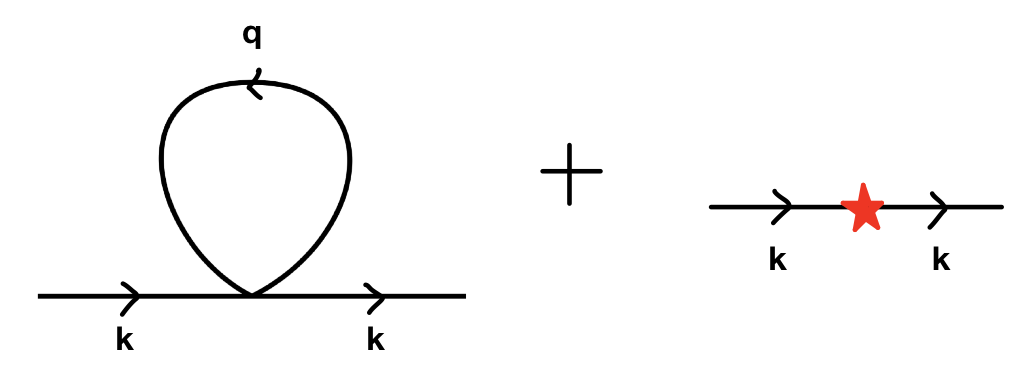
\includegraphics[align=c, width=0.35\linewidth]{pics/KG-3.png} \\
	&= i\Delta_0(k) \left[-\frac{g}{2}\int \frac{d^4 q}{(2\pi)^4} \frac{1}{q^2-m_R^2} + i(Ak^2-Bm_R^2) \right] i\Delta_0(k).
\end{aligned}
\end{equation}
Note that in the loop diagram, there is in total ($4 \times 3 = 12$) identical diagrams, and so gives the coefficients.
A simpler counter rule is that if the diagram has no symmetry, there is in total $4!$ identical diagrams and the denominator cancels out exactly, while for any remaining symmetries, the symmetry factor will remain in the denominator.
For the loop diagram we considered here, the symmetry factor is $2$.

Note that the second order correction to the Green's function has one ``ingoing'' leg and one ``outgoing'' leg, the core (or the amputated Green's function) in this case is called the \textit{self-energy} $i\Sigma(k^2)$:
\begin{equation}
	i\Sigma(k^2) = -\frac{g}{2}\int \frac{d^4 q}{(2\pi)^4} \frac{1}{q^4-m_R^2} + i(Ak^2-Bm_R^2).
\end{equation}
The integral is divergent, that when the counter terms come to rescue.
The divergent part of the integral can be absorbed into the coefficients, or be canceled by the counter terms.
In the following, we will see that the divergent integral
\begin{equation}
	I \equiv -\frac{g}{2} \int \frac{d^4 q}{(2\pi)^4} \frac{1}{q^4-m_R^2}
\end{equation}
can be regularized.
The regularization is typically controlled by a parameter which will recover the infinity when taking a specific limit.
The physical observable shall not depend explicitly on the regularization parameter, so the final result is free from divergent even if we take the limit.


\paragraph*{Regularization}
Consider the integral
\begin{equation}
	I = -\frac{g}{2} \int\frac{d \omega}{2\pi} \int\frac{d^3 q}{(2\pi)^3} \frac{1}{\omega^2 - \bm q^2-m_R^2 -i\varepsilon}.
\end{equation}
Since the singularity locates at $\pm(\sqrt{\bm q^2+m_R^2}-i\varepsilon)$, we can analytically change the integral of $\omega$ from real axis to the imaginary axis anti-clock-wisely, the result is equivalent to the substitution $\omega \rightarrow i\omega$.
The new integral is defined on the 4D Euclidean space:
\begin{equation}
	I = i \frac{g}{2} \int \frac{d^4 q}{(2\pi)^4} \frac{1}{q^2 + m_R^2}
	= i\frac{g}{2} \frac{\Omega_4}{(2\pi)^4} \int_0^\infty dq \ \frac{q^3}{q^2 + m^2_R},
\end{equation}
where $\Omega_d = 2 \pi^{d/2}/\Gamma\left(d/2\right)$ is the $d$-dimensional spherical area.

Till now the integral is essentially the same and thus still divergent.
Now we are going to regularize the expression.
One most frequently used regularization scheme is the \textit{dimensional regularization}.
It take note of the fact that the divergence of the integral only happens at integer dimension.
When we put the field theory to ($d=4-\varepsilon$)-dimensional space, the integral becomes:
\begin{equation}
	I_\varepsilon = i\frac{g\tilde{\mu}^\varepsilon}{2}\frac{\Omega_{4-\varepsilon}}{(2\pi)^{4-\varepsilon}} \int_0^\infty dq\ \frac{q^{3-\varepsilon}}{q^2+m_R^2}.
\end{equation}
Note that we have introduced a mass scale $\tilde\mu$ to get the correct dimensionality.
The integral is now convergent.
The specific form the the integral is not important, but we are concerned about the expansion near $\varepsilon = 0$. 
All the computation here can be done automatically (in \texttt{Mathematica}), and the result is
\begin{equation}
\begin{aligned}
	I_\varepsilon &= i\frac{g m_R^2}{32\pi^2} \left[\frac{2}{\varepsilon}+1+\log \left(\frac{4 \pi \tilde{\mu}^2 e^{-\gamma_E}}{m_R^2}\right)\right] + O(\varepsilon) \\
	&\equiv i\frac{g m_R^2}{32\pi^2} \left[\frac{2}{\varepsilon}+1+\log \left(\frac{\mu^2}{m_R^2}\right)\right] + O(\varepsilon),
\end{aligned}
\end{equation}
where $\gamma_E$ is the Euler constant. 
We have seen that the integral is controlled by the parameter $\varepsilon$.
In the $\varepsilon \rightarrow 0$ limit, the integral is divergent.


\paragraph*{Renormalization}
We are now going to renormalize the theory.
Note that in the self-energy definition
\begin{equation}
	\Sigma(k^2) = \frac{1}{i} I + A k^2-B^2 m_R^2,
\end{equation}
we have the freedom to choose the counter terms that cancel the infinity.
To the first order, the coefficients can be
\begin{equation}
	A = O(g^2), \quad
	B = \frac{g}{16\pi^2 \varepsilon} + O(g^2).
\end{equation}
The result is
\begin{equation}
	\Sigma(k^2) = \frac{g m_R^2}{16\pi^2} \log \left(\frac{\mu}{m_R}\right)
	+\frac{g m_R^2}{32\pi^2}+O(\varepsilon).
\end{equation}
The one-loop correction also leads to a infinite \textit{Dyson series}:
\begin{equation}
\begin{aligned}
	i\Delta(k) &= i\Delta_0(k) + i\Delta_0(k)\sum_{n=1}^\infty \left[i\Sigma(k^2)i\Delta_0(k)\right] \\
	&= \frac{i}{k^2 -m_R^2 + \Sigma(k^2)}.
\end{aligned}
\end{equation}



\paragraph*{Physical Observables}
The physical observable here is the rest mass $m_0$, which is experimentally measurable.
It equals to the pole of the propagator, i.e.,
\begin{equation}
	m_R^2 - \Sigma(m_0^2) = m_0^2.
\end{equation}
Depending on the mass scale $\mu$ we choose, the renormalized mass $m_R$ may or may not equal to the rest mass.
Specifically, we can choose mass scale so that $m_R = m_0$, that is
\begin{equation}
	\Sigma(m_0^2) = 0 \quad \Longrightarrow \quad
	\mu = e^{-\frac{1}{2}} m_0.
\end{equation}
To the first order, the self-energy has no momentum dependence, so there is no physical prediction.




\subsection{Second-order Correction to the Vertex}

Now consider the second order correction to the vertex function, which is the connected, amputated 4-point Green's function.
The perturbation correspond to 3 different Feynman diagrams together with a vertex counter term.
The explicit form is: 
\begin{equation}
\begin{aligned}
	i\Gamma_4(k_1,k_2,k_3,k_4) 
	&= 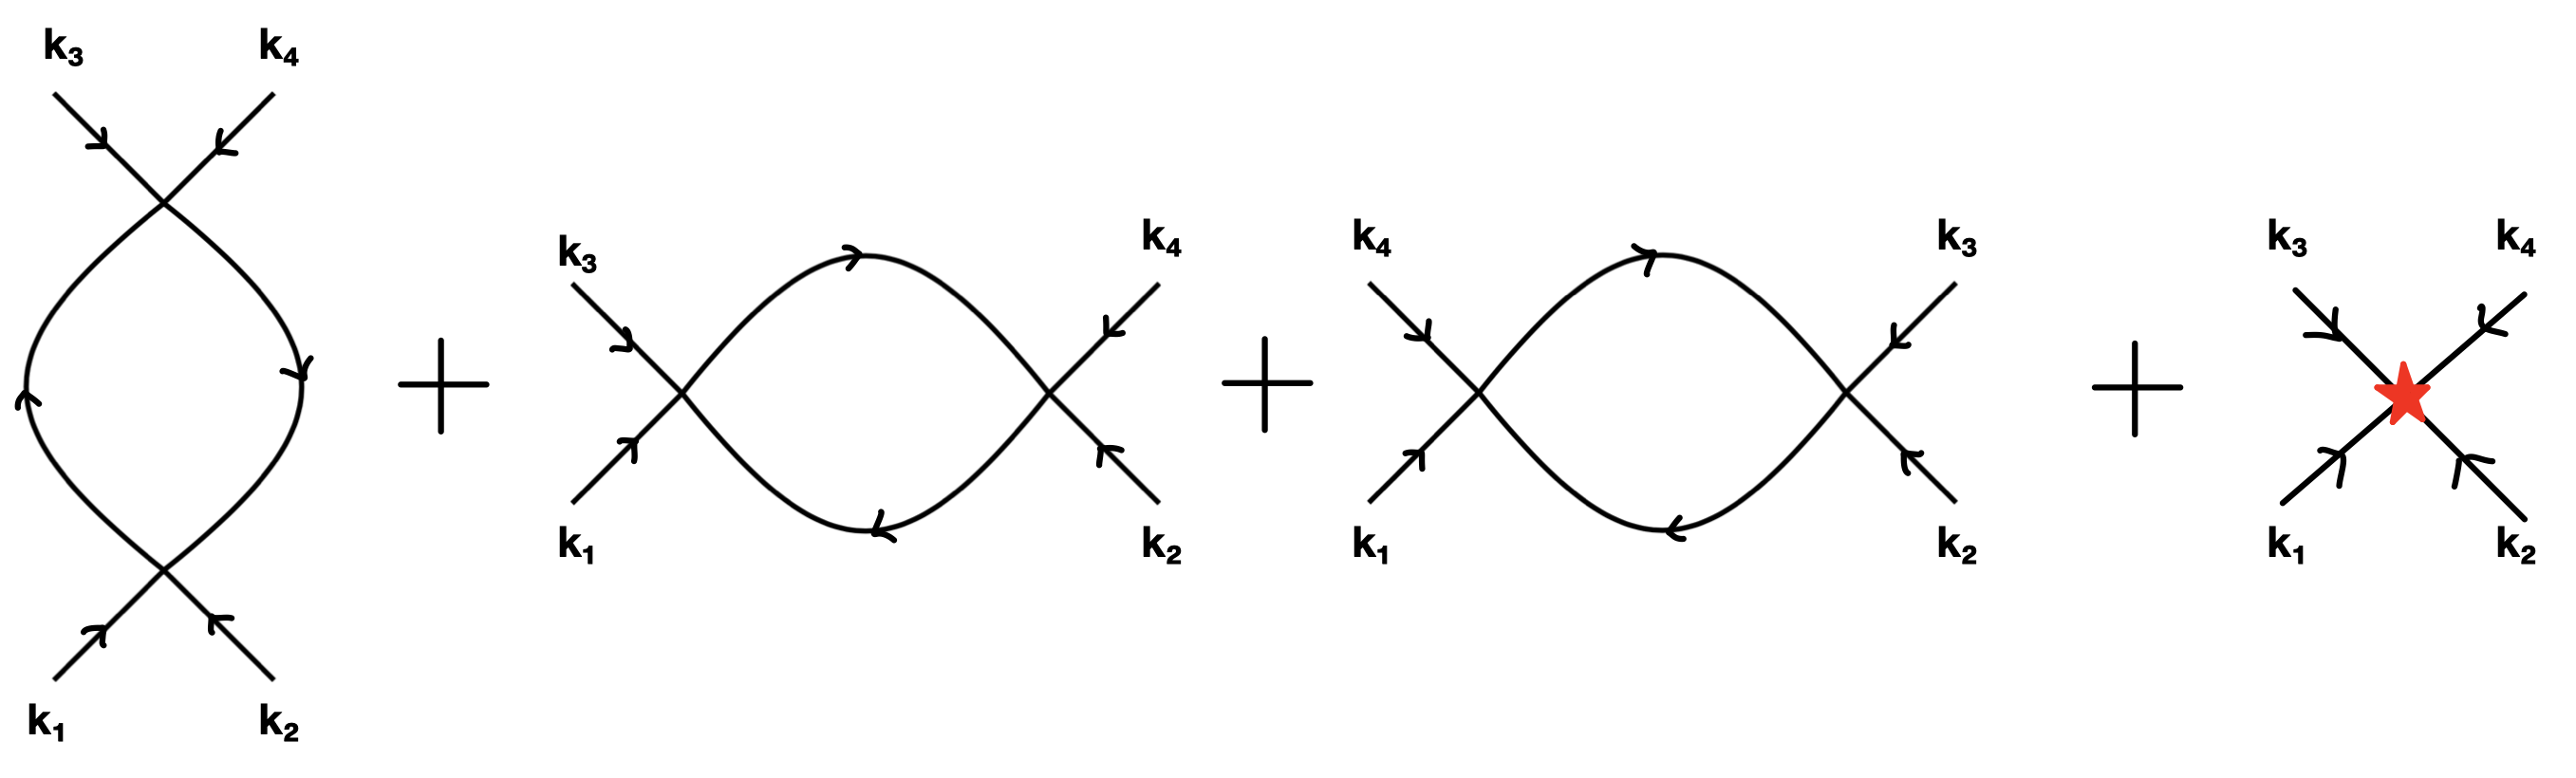
\includegraphics[align=c, width=0.6\linewidth]{pics/KG-4.png}\\
	&= \frac{g_R^2}{2} \left[iF(s)+iF(t)+iF(u)\right] -iCg_R,
\end{aligned}
\end{equation}
where we have introduced three momentum parameters $s$, $t$, and $u$: 
\begin{equation}
	s = (k_1+k_2)^2,\quad
	t = (k_1+k_3)^2,\quad
	u = (k_1+k_4)^2.
\end{equation}
The loop integrals for three channels are the same, denoted by
\begin{equation}
	iF(k^2) = \int \frac{d^4 q}{(2\pi)^4} \Delta_0(q) \Delta_0(q+k).
\end{equation}
The integral is again divergent.



\paragraph*{Regularization}
The denominator in the integral
\begin{equation}
	iF(k^2) = \int \frac{d^4 q}{(2\pi)^4} \frac{i}{q^2-m_R^2} \frac{i}{(q+k)^2-m_R^2}
\end{equation}
involves multiplication of two polynomial.
The expression can be simplified by the \textit{Feynman parametrization}, which is essentially the identity:
\begin{equation}
	\frac{1}{A_{1} \ldots A_{n}}=\int d F_{n}\left(x_{1} A_{1}+\ldots+x_{n} A_{n}\right)^{-n},
\end{equation}
where the integration measure over the Feynman parameters $x_{i}$ is
\begin{equation}
	\int d F_{n}=(n-1) ! \int_{0}^{1} d x_{1} \ldots d x_{n} \delta\left(x_{1}+\ldots+x_{n}-1\right).
\end{equation}
This measure is normalized so that $\int d F_{n} =1$. 
The simplest case is
\begin{equation}
	\frac{1}{A B}=\int_{0}^{1} \frac{dx}{[A+(B-A) x]^{2}}
	=\int_{0}^{1} \frac{\delta(x+y-1)}{[x A+y B]^{2}} dx dy.
\end{equation}
Other useful identities are
\begin{equation}
\begin{aligned}
	\frac{1}{A B^{n}} &=\int_{0}^{1} dxdy\frac{\delta(x+y-1)n y^{n-1}}{[x A+y B]^{n+1}} , \\
	\frac{1}{A B C} &=\int_{0}^{1} dxdydz \frac{2\delta(x+y+z-1)}{[x A+y B+z C]^{3}} .
\end{aligned}
\end{equation}

Using the Feynman parameters, the integral is
\begin{equation}
	iF(k^2) = \frac{i\Omega_4}{(2\pi)^4} \int_0^1 dx \int dq\ \frac{q^{3}}{\left[q^2+m_R^2+x(1-x)k^2\right]^2}.
\end{equation}
Using the dimensional regularization, the integral is
\begin{equation}
	iF_\varepsilon(k^2) = \frac{i\tilde{\mu}^{\varepsilon}\Omega_{4-\varepsilon}}{(2\pi)^{4-\varepsilon}} \int_0^1 dx \int dq\ \frac{q^{3-\varepsilon}}{\left[q^2+m_R^2+x(1-x)k^2\right]^2}.
\end{equation}
Then we carry out the calculation, the result is:
\begin{equation}
\begin{aligned}
	F_\varepsilon(s) &= \frac{1}{8\pi^2\varepsilon} + \frac{1}{16\pi^2}\int_0^1 dx \ln \left(\frac{4\pi \tilde{\mu}^2 e^{-\gamma_E}}{D_{s,x}}\right) \\
	&= \frac{1}{8\pi^2\varepsilon} +\frac{1}{8\pi^2}\ln \left(\frac{\mu}{m_R}\right) - \frac{1}{16\pi^2}\int_0^1 dx \ln\left(\frac{D_{s,x}}{m_R^2}\right),
\end{aligned}
\end{equation}
where we have denote
\begin{equation}
	D_{k^2,x} \equiv m_R^2+x(1-x)k^2.
\end{equation}
Now sum up the contribution from all channel, the result looks like:
\begin{equation}
	\Gamma^{(2)}_4 = \frac{3 g_R^2}{16\pi^2}\left[\frac{1}{\varepsilon} + \ln\left(\frac{\mu}{m_R}\right)\right] - \frac{g_R^2}{32\pi^2}\int_0^1 dx \ln\left(\frac{D_{s,x}D_{t,x}D_{u,x}}{m_R^6}\right)- C g_R.
\end{equation}


\paragraph*{Renormalization and Physical Observables}

To absorb the divergence, we can choose the counter term coefficient as
\begin{equation}
	C = \frac{3g_R}{16\pi^2}.
\end{equation}
So, to the second order, the vertex function is:
\begin{equation}
	\Gamma_4(k_1,k_2,k_3,k_4) = -g_R + \frac{g_R^2}{32\pi^2}\int_0^1 dx \ln\left(\frac{\mu^6}{D_{s,x}D_{t,x}D_{u,x}}\right).
\end{equation}
The vertex function is directly related to the physical observables.
It can be measured in the scattering experiment or just just by the repulsive force it generated.
We can choose the scale $\mu_0$ so that
\begin{equation}
	\Gamma(m_R,m_R,m_R,m_R) = -g_R.
\end{equation}
Then the corrected vertex function gives the physical predictions, for example on the scattering amplitude for different $k_i$'s.

\subsection{Renormalization Group}
Now consider the RG equation for the one-loop correction. 
The bare parameters are:
\begin{equation}
	g_0 = Z_g g\tilde{\mu}^{\varepsilon},\ 
	m_0 = Z_m^{1/2} m,
\end{equation}
The RG conditions are:
\begin{eqnarray}
	\frac{d g_0}{d\ln \mu}
	&=& \left(\frac{3}{16\pi^2 \varepsilon} + \frac{1}{g}\right)\frac{dg}{d\ln \mu} + \varepsilon = 0, \\
	\frac{d m_0}{d\ln \mu}
	&=& \frac{1}{32\pi^2 \varepsilon}\frac{dg}{d\ln \mu} + \frac{1}{m}\frac{dm}{d \ln \mu} = 0.
\end{eqnarray}
Consider the series expansion of beta function:
\begin{equation}
	\beta(g) = \frac{dg}{d\ln \mu} = \beta_1 g + \beta_2 g^2 +O(g^3).
\end{equation}
The beta function is
\begin{equation}
	\beta(g) = -\varepsilon g + \frac{3g^2}{16\pi^2} + O(g^3).
\end{equation}
The anomalous dimension of mass is
\begin{equation}
	\gamma_m = \frac{1}{m}\frac{dm}{d \ln \mu} = \frac{g}{32\pi^2}+O(g^2).
\end{equation}
One noticeable fact is that when we make the analytic continuation to $\varepsilon>0$, the betta function predict a nontrivial fixed point at
\begin{equation}
	g^*_{\mathrm{WF}} = \frac{16\pi^2 \varepsilon}{3}.
\end{equation}
This fixed point is called the \textit{Wilson-Fisher fixed point}, and is related to the ferromagnetic-paramagnetic transition.



\section{Wilsonian Renormalization Group}

In this section, we consider another regulation scheme from Wilson's perspective.
We introduce a UV cutoff for the theory, and the action for $\phi^4$ theory is
\begin{equation}
	S[\phi] = \int_{|k|<\Lambda} \frac{d^d k}{(2\pi)^d}\left[\frac{1}{2} \left(k^2-r(\Lambda)\right)\phi^2 - \frac{1}{4!}g(\Lambda)\phi^4\right].
\end{equation}
We choose to fix the coefficient of the kinetic term.
The mass and coupling constant is dependent of the energy scale $\Lambda$.
The course graining makes $k \rightarrow s k$.
In the momentum domain, we split the field into slow and fast parts $\phi = \phi_{s} + \phi_{f}$, integrate the fast momentum part $\Lambda/s<|k|<\Lambda$, rescale the field strength, and obtain new effective theory.




\subsection{Integral over Energy Shell}

We first consider the one-loop correction:\footnote{In this section, the field theory is defined on the Euclidean space.}
\begin{equation}
	e^{-S'[\phi_{\mathrm{s}}]} = \int D[\phi_{\mathrm{f}}] e^{-S[\phi_{\mathrm{s}}+\phi_{\mathrm{f}}]}.
\end{equation} 
The action can be decomposed into the fast field part, slow field past, and the interacting part:
\begin{equation}
	S[\phi_{\mathrm{s}}+\phi_{\mathrm{f}}] = S[\phi_{\mathrm{s}}] + S[\phi_{\mathrm{f}}] + S[\phi_{\mathrm{s}}, \phi_{\mathrm{f}}].
\end{equation}
In the $\phi^4$ case, the only relevant part of the action is
\begin{equation}
	S[\phi_{\mathrm{s}},\phi_{\mathrm{f}}] = \frac{g}{4} \int d^d x\ \phi_{\mathrm{s}}^2 \phi_{\mathrm{f}}^2 + \cdots
\end{equation}
The effective action for the slow field can be obtained by integrate out the fast field.
To the second order,
\begin{equation}
\begin{aligned}
	\exp\left(-S'[\phi_{\mathrm{s}}]\right) 
	&= e^{-S[\phi_{\mathrm{s}}]} \left[1-\langle S[\phi_{\mathrm{s}},\phi_{\mathrm{f}}]\rangle_f + \frac{1}{2} \langle S[\phi_{\mathrm{s}},\phi_{\mathrm{f}}]\rangle^2+O(g^3) \right]\\
	&= \exp\left[-S[\phi_{\mathrm{s}}]-\langle S[\phi_{\mathrm{s}},\phi_{\mathrm{f}}]\rangle_f + \frac{1}{2}\langle S[\phi_{\mathrm{s}},\phi_{\mathrm{f}}]^2\rangle^c_f +O(g^3)\right].
\end{aligned}
\end{equation}
This produce a new action with different coefficients, and possibly new terms.
In the renormalization group sense, we only need to keep track of the coefficients of the relevant terms.\footnote{Although the irrelevant terms vanishes during the RG flow, they may contributes back to the relevant terms and thus influence the RG flow. However, this process is captured by higher order perturbation theory. So in practice, we just ignore all the diagram producing irrelevant terms.}
After proper renormalization, the coupling constant can alter in the coarse-graining process.


\subsection{RG-Flow of Phi-4 Theory}

The first order perturbation contribute to the mass term:
\begin{equation}
\begin{aligned}
	\left\langle S\left[\phi_{\mathrm{s}}, \phi_{\mathrm{f}}\right]\right\rangle_{\mathrm{f}}
	= 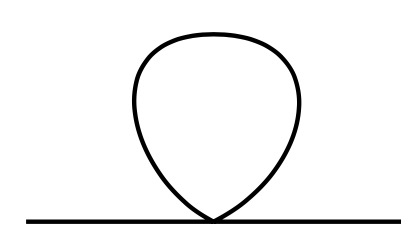
\includegraphics[align=c,width=0.1\linewidth]{pics/RG-1.jpg} 
	=\frac{g}{4} \int_{d\Lambda} \frac{d^d q}{(2 \pi)^d} \frac{1}{r+q^{2}} \int_{|k|<\Lambda/s} \frac{d^d k}{(2 \pi)^{d}} \phi_{\mathrm{s}}(k) \phi_{\mathrm{s}}(-k).
\end{aligned}
\end{equation}
We are interested in the RG-flow in the vicinity of the critical point. 
So we can calculate the coefficient perturbatively for $r$:
\begin{equation}
	\int_{d\Lambda} \frac{d^d q}{(2 \pi)^d} \frac{1}{r+q^{2}}
	= \int_{d\Lambda}\frac{d^d q}{(2 \pi)^d} \left(\frac{1}{q^2} - \frac{r}{q^4}\right)
	= \Omega_d \left[\frac{1-s^{2-d}}{d-2} - \frac{r\left(1-s^{4-d}\right)}{d-4}\right],
\end{equation} 
where $\Omega_{d}=\left(2 \pi^{d / 2} / \Gamma(d / 2)\right) /(2 \pi)^{d} $ denotes the volume of the $d$-dimensional unit sphere.
Note that we used $\Lambda$ as the unit, since it is the only natural scale of the theory.
After the energy-shell integral, we should also renormalize the theory.
To restore the energy shell back to $1$, we change the variable as $k'=sk$, which left an additional $s^{-d-2}$ factor in the kinetic term.
Therefore we renormalize the field as $\phi \rightarrow s^{d/2+1}\phi$.
Take all things into account, and set the infinitesimal variable as $s=e^{dl}$, we get the RG flow of $r$ as
\begin{equation}
\begin{aligned}
	dr &\rightarrow s^2\left[r+\frac{g \Omega_{d}}{2(d-2)}\left(1-s^{2-d}\right)-\frac{r g \Omega_{d}}{2(d-4)}\left(1-s^{4-d}\right)\right]-r \\
	&\simeq (1+2dl) \left[r+ \frac{1}{2} g \Omega_{d} dl - \frac{1}{2} r g \Omega_{d} dl \right]-r \\
	&\simeq \left(2r+ \frac{1}{2}g\Omega_d -\frac{1}{2}rg\Omega_d \right)dl.
\end{aligned}
\end{equation}
We assume the dimension is $d=4-\varepsilon$ and the result to the lowest order of $\varepsilon$.
For the RG-flow of the parameter $r$, we expand to the zeroth order of $\varepsilon$, $\Omega_{4-\varepsilon} \approx \Omega_{4}=\frac{1}{8 \pi^{2}}$, and the result is
\begin{equation}
	\frac{dr}{dl} = 2r+ \frac{g}{16\pi^2} -\frac{rg}{16\pi^2}.
\end{equation}

Then we turn to the second order perturbation, which correct the vertex:\footnote{Note that the most general vertex function is momentum dependent: $g=g(k_1,k_2,k_3,k_4)$. While near $d=4$, the momentum dependent part of the vertex function is irrelevant. We thus only consider the loop correction with zero net external momentum.}
\begin{equation}
	\frac{1}{2}\left\langle S\left[\phi_{\mathrm{s}}, \phi_{\mathrm{f}}\right]^{2}\right\rangle^c_{\mathrm{f}} 
	= 
\includegraphics[align=c,width=0.15\linewidth]{pics/RG-2.jpg} 
	= \frac{g^{2}}{16} \int_{d\Lambda} \frac{d^{d} q}{(2 \pi)^{d}} \frac{1}{\left(r+q^{2}\right)^{2}} \left(\int d^{d} r\  \phi_{\mathrm{s}}^{4}\right).
\end{equation}
Similarly, the energy shell integral is
\begin{equation}
	\int_{d\Lambda} \frac{d^{d} q}{(2 \pi)^{d}} \frac{1}{\left(r+q^{2}\right)^{2}}
	= \int_{d\Lambda} \frac{d^{d} q}{(2 \pi)^{d}} \left(\frac{1}{q^4}-\frac{2r}{q^6} \right)
	= \Omega_d\left[\frac{1-s^{4-d}}{d-4}-\frac{2r(1-s^{6-d})}{d-6}\right].
\end{equation}
The RG-flow of $g$ is
\begin{equation}
\begin{aligned}
	dg &\rightarrow s^{(4-d)}\left[g - \frac{3g^2\Omega_d}{2(d-4)}(1-s^{4-d})+\frac{3rg^2\Omega_d}{d-6}(1-s^{6-d})\right]-g \\
	&\simeq [1+(4-d)dl] \left[g - \frac{3}{2} g^2\Omega_d dl + 3rg^2\Omega_d dl \right]-g \\
	&\simeq \left[(4-d)g-\frac{3}{2} g^2(1-2r)\Omega_d \right]dl.
\end{aligned}
\end{equation}
The beta function for lowest order $\varepsilon$-expansion is
\begin{equation}
	\frac{dg}{dl} = \varepsilon g - \frac{3g^2}{16\pi^2} + \frac{6 r g^2}{16\pi^2}.
\end{equation}

\begin{figure}[]
	\centering
	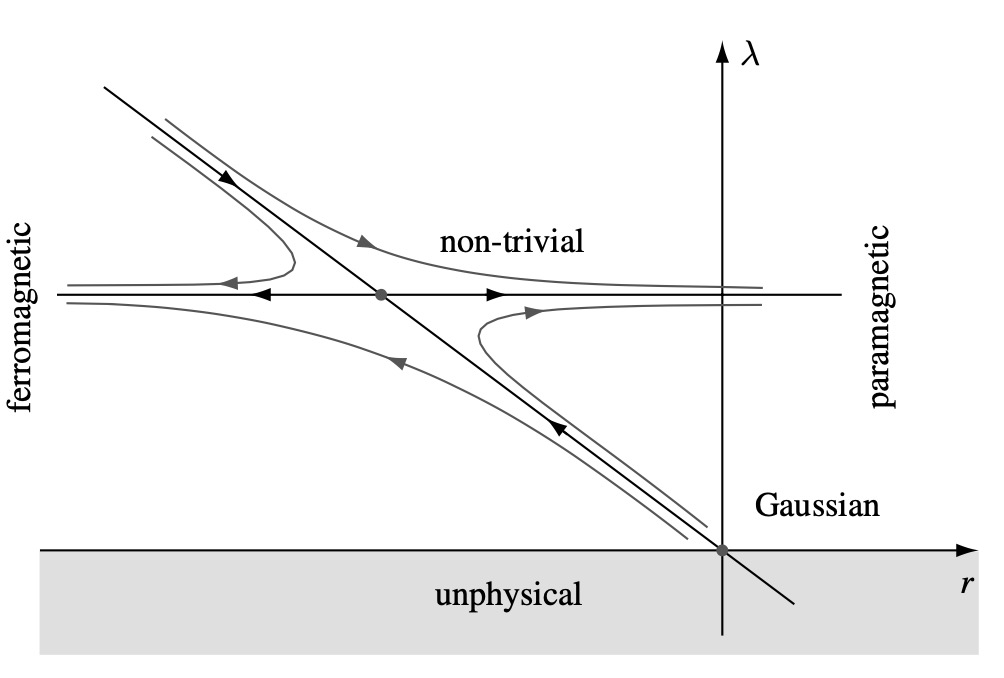
\includegraphics[hsmash=c,width=0.35\linewidth]{pics/RG-flow.jpg}
	\caption{Phase diagram of the $\phi^4$-model as obtained from the $\varepsilon$-expansion.}
	\label{fig:rg-flow}
\end{figure}

The Gaussian fixed point and the nontrivial Wilson-Fisher fixed point determined the phase diagram of the $\phi^4$ model.
As shown in Fig.~\ref{fig:rg-flow}, there are a disordered paramagnetic phase and an ordered ferromagnetic phase.
The ordered-disordered transition is the result of spontaneous symmetry breaking.




\section{Spontaneous Symmetry Breaking}

In this section, we consider the effective field theory for the spontaneous symmetry-breaking phase.
We first consider the real $\phi^4$ theory with $Z_2$ symmetry, then discuss the complex scalar field with continuous symmetry breaking.

\subsection{Spontaneous Breaking of $Z_2$ Symmetry}
The ferromagnetic phase corresponds to the $\phi^4$ Lagrangian with the minus mass term:
\begin{equation}
	\mathcal L =\frac{1}{2}\partial^\mu \phi \partial_\mu \phi +\frac{m^2}{2}\phi^2 - \frac{g}{4!}\phi^4.
\end{equation}
The energy is minimized by the nonzero field configuration
\begin{equation}
	\phi_0 = \pm \sqrt{\frac{6m^2}{g}}.
\end{equation}
To describe the low energy behavior, we just need to expand the field around on of the minima: $\phi = \phi_0 +\tilde\phi$.
Then the effective theory is
\begin{equation}
	\mathcal{L}=\frac{1}{2} \partial_{\mu} \tilde{\phi}\partial^{\mu} \tilde{\phi} -m^{2} \tilde{\phi}^{2}-\sqrt{\frac{g}{6}} m \tilde{\phi}^{3}-\frac{g}{4 !} \tilde{\phi}^{4}+\frac{3 m^{4}}{2 g}.
\end{equation}
We see that the effective theory is an ordinary Klein-Gordon field with both $\phi^3$ and $\phi^4$ interaction present.
The original $Z_2$ symmetry $\phi \rightarrow -\phi$ is spontaneously broken. 


\subsection{Spontaneous Breaking of U(1) Symmetry}
Now we generalized the discussion the complex $\phi^4$ theory:
\begin{equation}
	\mathcal L = \partial^\mu \phi^* \partial_\mu \phi + m^2\phi^* \phi - \frac{g}{4}(\phi^*\phi)^2.
\end{equation}
The minimal energy field configuration is 
\begin{equation}
	|\phi_0|^2 = \frac{2m^2}{g}.
\end{equation}
The field can be parameterized as
\begin{equation}
	\phi(x)=\left[\sqrt{\frac{2 m^{2}}{g}}+\frac{\sigma(x)}{\sqrt{2}} \right] \exp\left[{i \frac{\pi(x)}{F_{\pi}}}\right],
\end{equation}
with $F_{\pi}$ a real number. 
Expanding the Lagrangian around the minimum we find
\begin{equation}
	\mathcal{L}= \frac{2m^2/g}{F_\pi^2} \left[1+\frac{\sqrt{g}}{2m} \sigma(x) \right]^{2} \left(\partial_{\mu} \pi\right)^{2} +\frac{1}{2}\left(\partial_{\mu} \sigma\right)^{2}
	-\left(m^{2} \sigma^{2}+\frac{\sqrt{g} m}{2} \sigma^{3}+\frac{g}{16} \sigma^{4}\right)+\frac{m^{4}}{g}.
\end{equation}
Choosing $F_\pi = 2m/\sqrt{g}$, the $\pi$ mode is canonically normalized.
This theory is called a \textit{linear sigma model}.
The massless $\pi$ field is the Goldstone boson.








\end{document}


